\documentclass[UTF8,aspectratio=169,mathserif]{beamer}
\usepackage{ctex}
\usepackage{ulem}
\usepackage{color}
\usepackage{amssymb}
\usepackage{amsmath}
\usetheme{Berlin}
\setbeamertemplate{navigation symbols}{}

\title{5 - 多项式层级和交替}
\subtitle{The polynomial hierarchy and alternations}
\author{报告人:许博}
\date{\today}

\begin{document}
	
	\begin{frame}
		\titlepage
	\end{frame}
	
	\begin{frame}{目录}
		\tableofcontents
	\end{frame}
	
	\section{类 ${\bf\Sigma}_2^p$}
	\begin{frame}{似乎不能被 $\bf NP$-完全捕获的计算问题}
		\begin{block}{INDSET (NP-Complete)}
			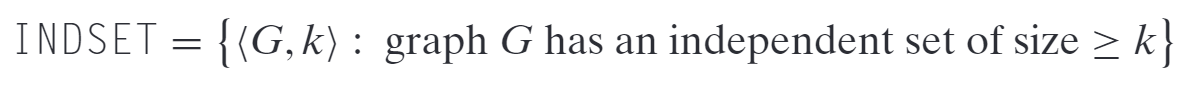
\includegraphics[width=0.6\linewidth]{../5 & 6/note.assets/image-20210426152232421.png}
		\end{block}
		
		\begin{block}{EXACT INDSET}
			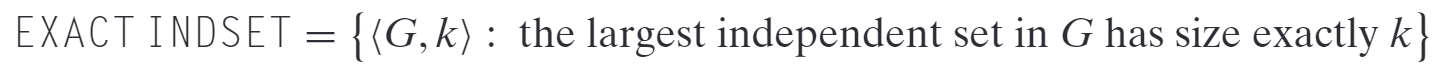
\includegraphics[width=0.7\linewidth]{../5 & 6/note.assets/image-20210426152349887.png}
		\end{block}
		
		\begin{block}{MIN-EQ-DNF}
			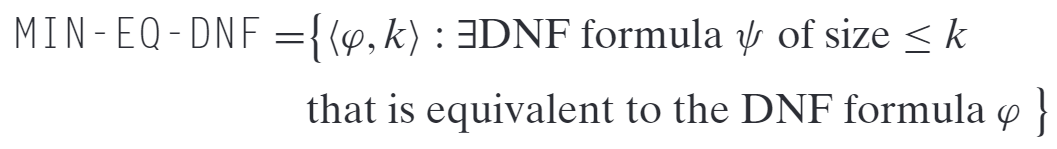
\includegraphics[width=0.6\linewidth]{../5 & 6/note.assets/image-20210426152757453.png}
			
			其中 a DNF formula is a Boolean formula that is an OR of ANDs 
		\end{block}
	\end{frame}
	
	\begin{frame}{定义类 ${\bf\Sigma}_2^p$}
		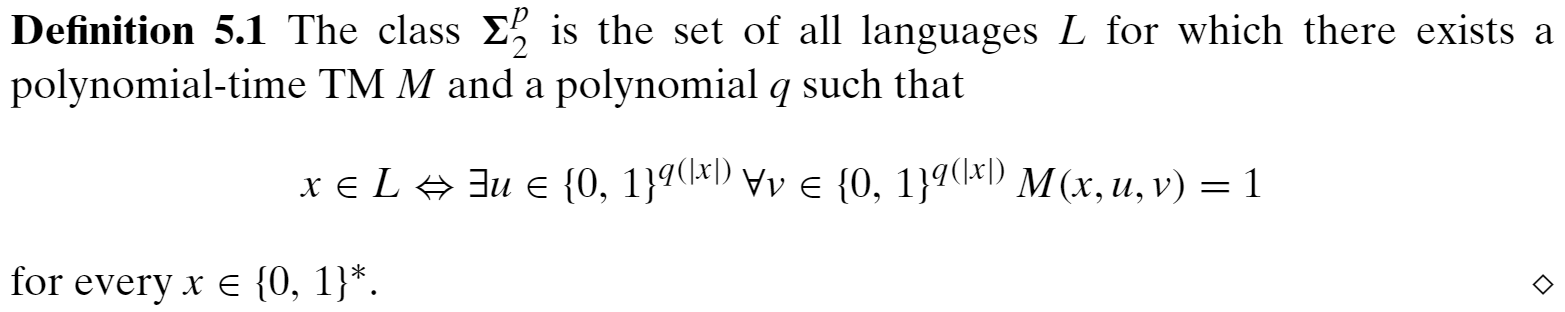
\includegraphics[width=\linewidth]{../5 & 6/note.assets/image-20210426154842170.png}\newline
		
		1. ${\bf\Sigma}_2^p$ 包含(但不只包含)类 $\bf NP$ 和 $\bf coNP$;
		
		2. MIN-EQ-DNF 是 ${\bf\Sigma}_2^p$-完全问题。
	\end{frame}
	
	\section{多项式层级}
	\begin{frame}{$\bf PH$ 的定义}
		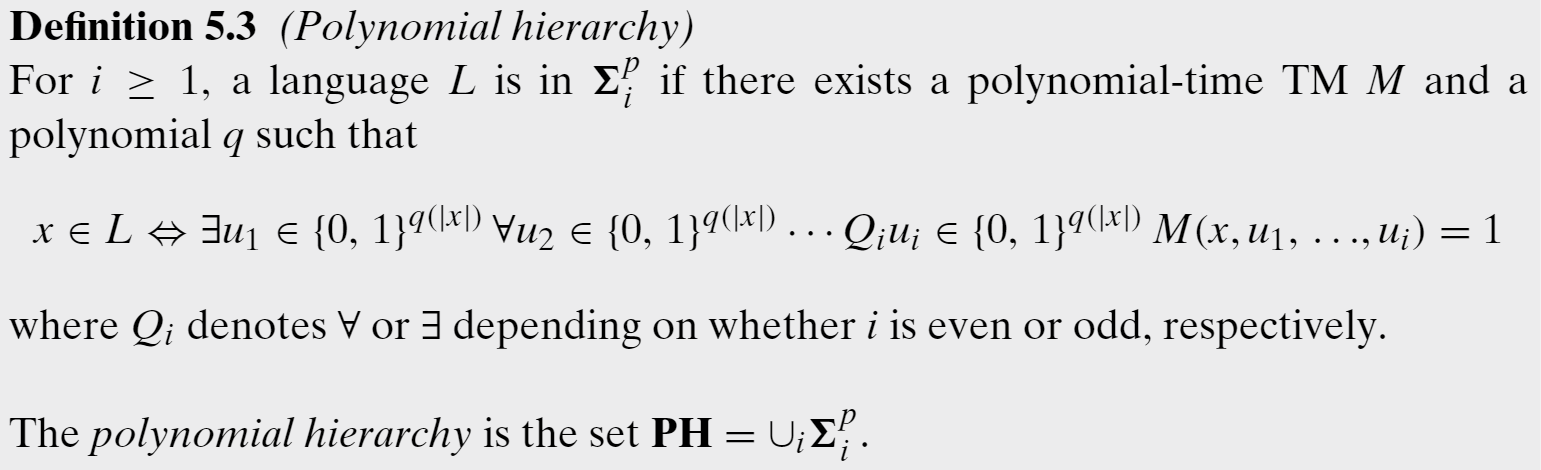
\includegraphics[width=\linewidth]{../5 & 6/note.assets/image-20210426160324184.png}\newline
		
		定义 ${\bf\Pi}_i^p={\bf co\Sigma}_i^p=\{\overline{L}:L\in{\bf\Sigma}_i^p\}$。有 ${\bf\Sigma}_1^p={\bf NP}$。因此 ${{\bf\Pi}_1^p={\bf coNP}}$。
		
		并且有 ${\bf\Sigma}_i^p \subseteq{\bf\Pi}_{i+1}^p\subseteq{\bf\Sigma}_{i+2}^p$,因此${\bf PH}=\cup_{i>0}{\bf\Pi}_i^p$。
	\end{frame}
	
	\begin{frame}{$\bf PH$ 的性质}
		塌缩(collapse):如果存在 $i$ 使得 ${{\bf\Sigma}_i^p}={{\bf\Sigma}_{i+1}^p}$,则称 PH 塌缩,同时隐含 ${{\bf\Sigma}_i^p}={\cup}_{j\ge1}{{\bf\Sigma}_j^p}={\bf PH}$,这时可以说 PH 塌缩至第 $i$ 层。\newline
		
		“PH 不塌缩” 是 $\bf P\neq NP$ 以及 $\bf NP\neq coNP$ 猜想的一般形式。\newline
		
		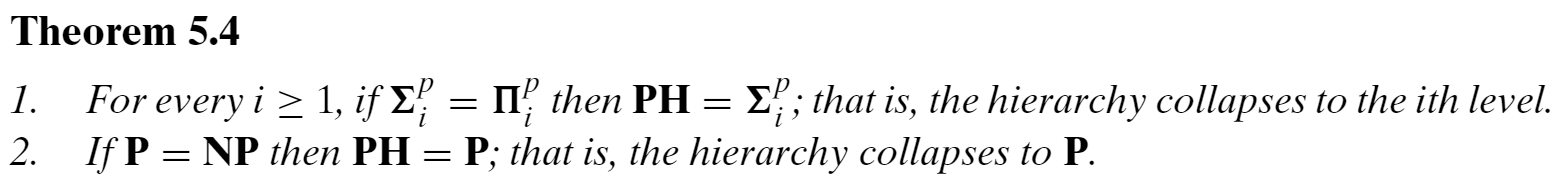
\includegraphics[width=\linewidth]{../5 & 6/note.assets/image-20210427092228569.png}
	\end{frame}
	
	\begin{frame}{$\bf PH$ 不同层的完全问题}
		每个 $i\in\mathbb{N}$,${{\bf\Sigma}_i^p}$ 和 ${{\bf\Pi}_i^p}$ 都有完全问题,PH 没有完全问题(除非 PH 塌缩)\newline
		
		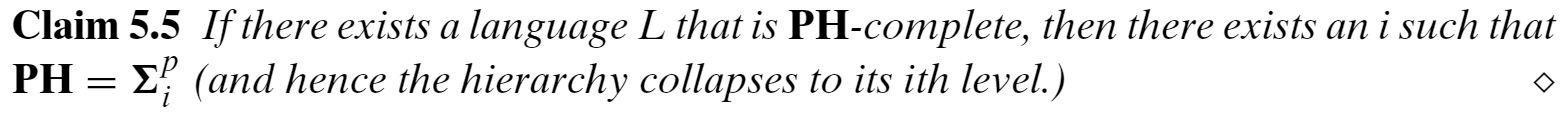
\includegraphics[width=\linewidth]{../5 & 6/note.assets/image-20210427092442758.png}\newline
		
		如 $\bf NP$ 和 $\bf coNP$,$\bf PH$ 也包含于 $\bf PSPACE$。而除非 PH 塌缩,否则 $\bf PH\neq PSPACE$
	\end{frame}
	
	\begin{frame}
		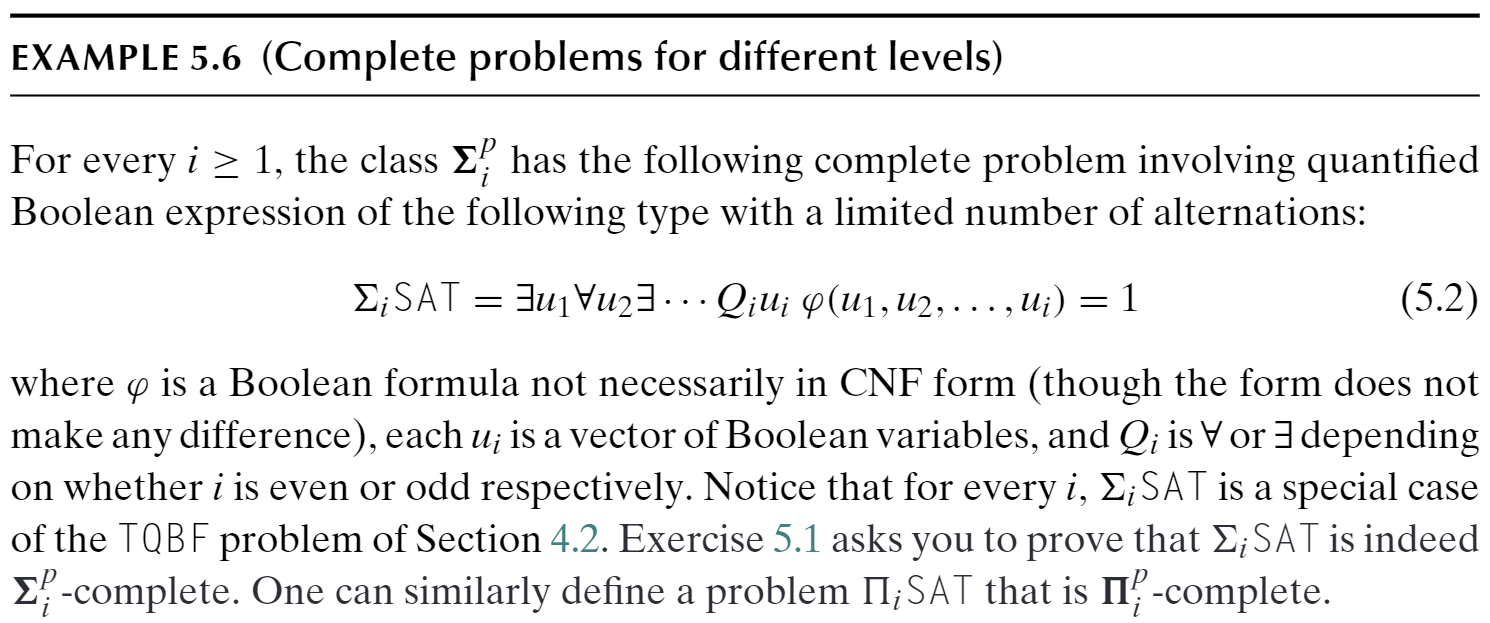
\includegraphics[width=\linewidth]{../5 & 6/note.assets/image-20210427093527360.png}\newline
		
		需要注意的是,其中每个 $u_i$ 表示一组布尔变量。
	\end{frame}
	
	\section{交替图灵机}
	\begin{frame}{交替图灵机(Alternating TM)的定义}
		NDTM 不是一个现实的计算模型,但它有助于我们关注猜一个答案和验证它的区别。ATM 在没有明显的短证明的问题中起到类似的作用。\newline
		
		ATM 类似 NDTM,但其内部状态(除了接受和终止状态)会被 $\exists$ 或者 $\forall$ 标记。NDTM 接受输入当存在一条到达接受状态的路径时,可以看作每个内部状态都标记为 $\exists$,在 ATM 中,则可以在 $\exists$ 和 $\forall$ 之间交替选择。
	\end{frame}
	\begin{frame}
		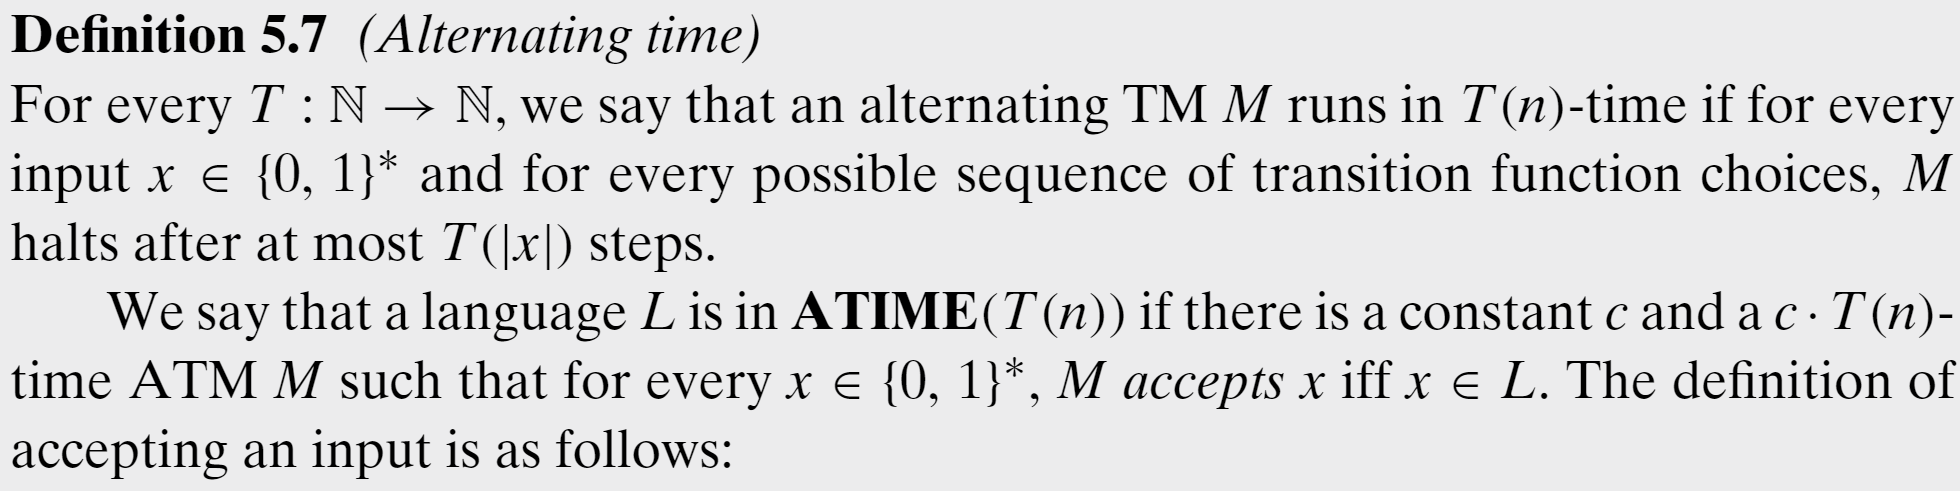
\includegraphics[width=\linewidth]{../5 & 6/note.assets/image-20210427213236953.png}\newline
		
		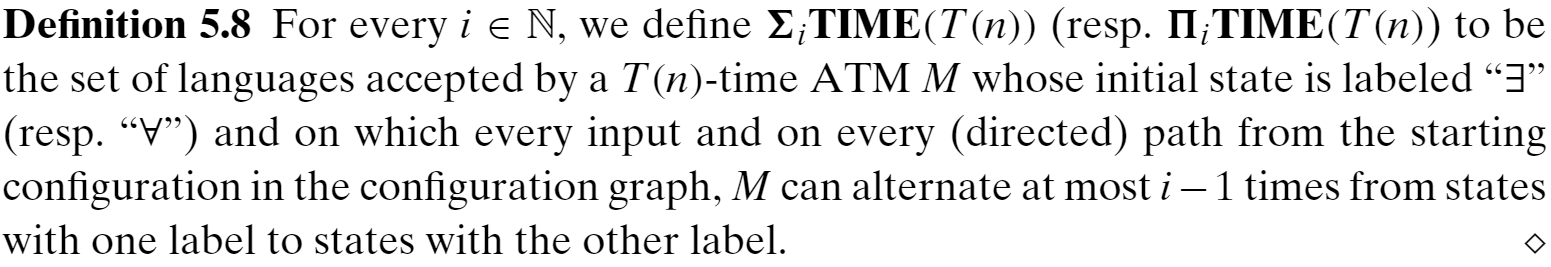
\includegraphics[width=\linewidth]{../5 & 6/note.assets/image-20210427094554653.png}
	\end{frame}
	
	\section{通过预言机定义层级}
	\begin{frame}
		\begin{columns}
			\begin{column}{0.48\textwidth}
				\begin{exampleblock}{定义4.4.1(形成规则,formation rule)}
					(form)\ $\dfrac{\Gamma\vdash A:s\ \ \ \Gamma\vdash B:s}{\Gamma\vdash A\rightarrow B:s}$
				\end{exampleblock}
			\end{column}
			\begin{column}{0.48\textwidth}
				\begin{block}{定义3.4.7($\lambda{\rightarrow}$中的形成规则,formation rule in $\lambda{\rightarrow}$)}
					(form) 如果$\Gamma$是一个$\lambda{2}$-上下文,$B\in\mathbb{T}2$且$B$中所有的自由类型变量已经在$\Gamma$中声明,则$\Gamma\vdash B:*$
				\end{block}
			\end{column}
		\end{columns}
		
		三个$s$同时表示*或$\square$。
		
		在引入新的(form)规则之前,由(var)规则与(weak)规则只能推导出$*:\square,\alpha:*,x:\alpha$而不能推出箭头类型$*\rightarrow*:\square$以及$\alpha\rightarrow\beta:*$等。
		
		\begin{block}{例子}
			$\dfrac{\emptyset\vdash*:\square\ \ \ \emptyset\vdash*:\square}{\emptyset\vdash*\rightarrow*:\square}\ (form)$
		\end{block}
		
	\end{frame}
	
	\section{SAT 的时间-空间权衡}
	\begin{frame}
		\begin{columns}
			\begin{column}{0.48\textwidth}
				\begin{exampleblock}{应用规则,application rule}
					(appl) $\dfrac{\Gamma\vdash M:A\rightarrow B\ \ \ \Gamma\vdash N:A}{\Gamma\vdash MN:B}$
				\end{exampleblock}
			\end{column}
			\begin{column}{0.48\textwidth}
				\begin{exampleblock}{抽象规则,abstraction rule}
					(abst) $\dfrac{\Gamma,x:A\vdash M:B\ \ \ \Gamma\vdash A\rightarrow B:s}{\Gamma\vdash\lambda x:A.M:A\rightarrow B}$
				\end{exampleblock}
			\end{column}
		\end{columns}
		
		\hspace*{\fill} \\
		
		$\lambda{\uline{\omega}}$中的这两个规则与之前略有不同:
		
		\begin{itemize}
			\item 用于类型的元变量(meta-variable)的名字不同,因为$\lambda{\uline{\omega}}$中的类型更为通用
			
			\item 需要保证类型是良构的(即可以由上下文推导出)
		\end{itemize}
		
		当$s\equiv*$时,$A\rightarrow B$是一个第二层的类型,如$(\alpha\rightarrow\beta)\rightarrow\gamma$,
		
		当$s\equiv\square$时,$A\rightarrow B$就是一个第三层的类(kind),如$(*\rightarrow*)\rightarrow*$。
	\end{frame}
	
	
	
\end{document}